\documentclass[oneside,final,14pt,a4paper]{extreport}

\usepackage{tempora} % Times New Roman alike font  

\usepackage{vmargin}
\setpapersize{A4}
\setmarginsrb{2.5cm}{2.2cm}{2.2cm}{2.2cm}{0pt}{10mm}{0pt}{13mm}
\usepackage{setspace}
\setstretch{1.5}
\usepackage{indentfirst}
\parindent=1.25cm

%%%%% ADDED TO SUPPORT TT BOLD FACES %%%%
\DeclareFontShape{OT1}{cmtt}{bx}{n}{<5><6><7><8><9><10><10.95><12><14.4><17.28><20.74><24.88>cmttb10}{}
\renewcommand{\ttdefault}{pcr}
%%%%% END %%%%%%%%%%%%%%%%%%%%%%%%%%%%%%% 

\usepackage{atbegshi,picture}
\usepackage[T1,T2A]{fontenc}
\usepackage[utf8]{inputenc}

\usepackage[english]{babel}
\usepackage[backend=biber,style=ieee,autocite=inline]{biblatex}
\addbibresource{ref.bib}
\DefineBibliographyStrings{english}{%
  bibliography = {References},}
\usepackage{blindtext}

\usepackage{pdfpages}
\newenvironment{bottompar}{\par\vspace*{\fill}}{\clearpage}
\usepackage{amsmath,amsfonts}
\usepackage{url}
\usepackage{amsthm}
\newtheorem{theorem}{Theorem}
\newtheorem{corollary}{Corollary}
\newtheorem{lemma}{Lemma}
\newtheorem{proposition}{Proposition}
\theoremstyle{definition}
\newtheorem{definition}{Definition}
\theoremstyle{remark}
\newtheorem*{remark}{Remark}
\theoremstyle{remark}
\newtheorem*{example}{Example}

\usepackage{float}
\usepackage{graphicx}
\graphicspath{{figs/}} %path to images
\usepackage{array}
\usepackage{multirow,array}
\usepackage{caption}
\usepackage{subcaption}
\usepackage{hyperref}
\hypersetup{colorlinks=true, linkcolor=black, citecolor=black}
\usepackage{paralist}
\usepackage{listings}
\usepackage{zed-csp}
\usepackage{fancyhdr}
\usepackage{csquotes}
\usepackage{color}

\usepackage{chngcntr}
\usepackage{upgreek} 
\usepackage{bm}
\usepackage{booktabs}
\usepackage{longtable}
\usepackage[font=singlespacing, labelfont=bf]{caption}
\newcommand\pic[1]{(Fig. \ref{#1})}
\newcommand\tab[1]{(Tab. \ref{#1})}

\setlength{\headheight}{32.0976pt}
\usepackage{enumitem}
\newlist{inlinelist}{enumerate*}{1}
\setlist*[inlinelist,1]{label=(\arabic*),}

\captionsetup[table]{labelfont={normalfont}, name={TABLE}, labelsep={newline}}
\setlength{\parindent}{2em} 
\DeclareCaptionLabelSeparator{figSep}{.\quad}
\captionsetup[figure]{labelfont={normalfont}, name={Fig.}, labelsep=period}
\counterwithin{figure}{chapter}

\usepackage{placeins}

\pagestyle{fancyplain}
\renewcommand{\chaptermark}[1]{\markboth{\chaptername~\thechapter~--~#1}{}}
\renewcommand{\sectionmark}[1]{\markright{\thesection\ #1}}
\rhead[\fancyplain{}{\bf\leftmark}]{\fancyplain{}{\bf\thepage}}
\lhead[\fancyplain{}{\bf\thepage}]{\fancyplain{}{\bf\rightmark}}
\cfoot{}

\newcommand{\dedication}[1]{%
   \thispagestyle{empty}
   \begin{flushleft}\raggedleft #1\end{flushleft}
}

\begin{document}

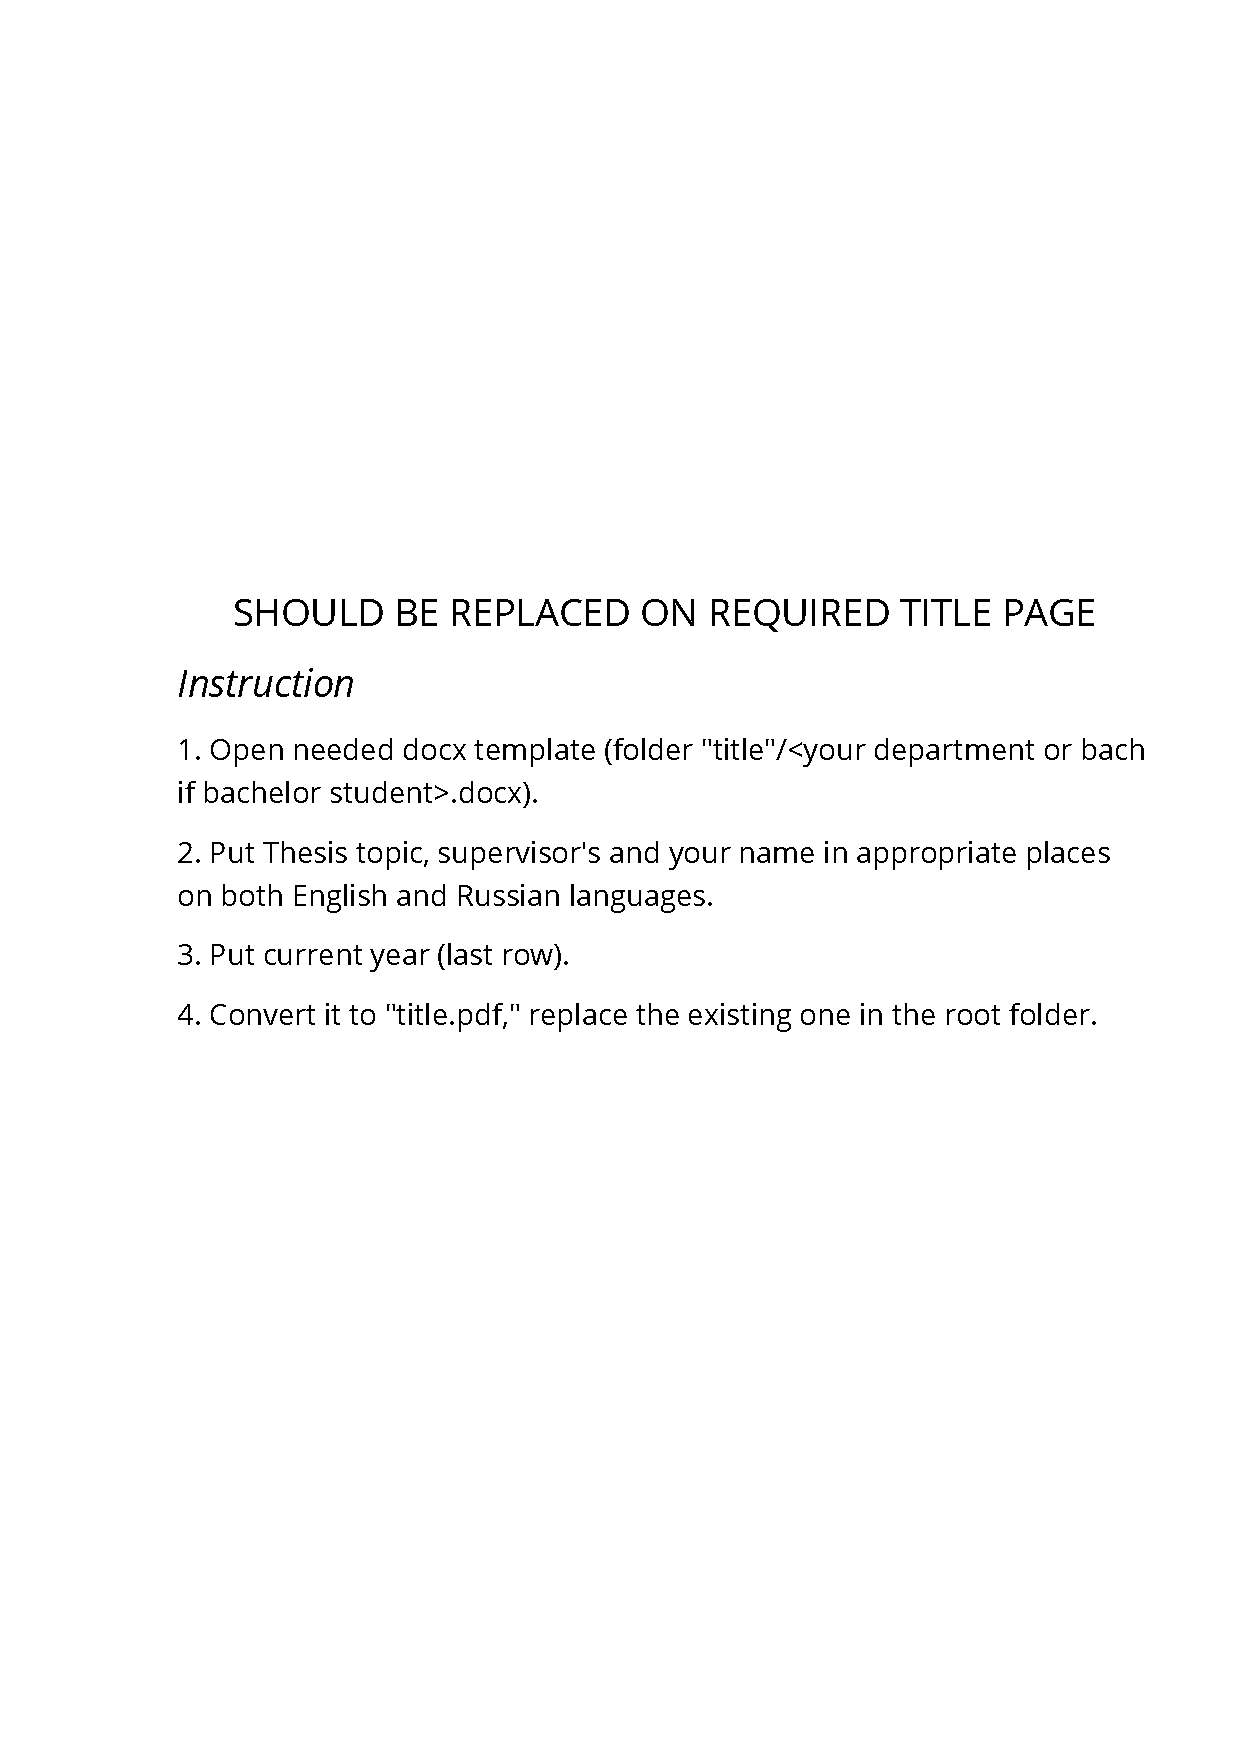
\includepdf[pages=-]{title.pdf}
\tableofcontents
\listoftables
\listoffigures
\newpage

\begin{abstract}
% skip one line to make the abstract start with indent

My abstract starts from here.
\end{abstract}
\setcounter{page}{7}

\chapter{Introduction}
\label{chap:intro}
\chaptermark{Optional running chapter heading}

\blindtext

\chapter{Literature Review}
\label{chap:lr}

\blindtext

\chapter{Methodology}
\label{chap:met}

Referencing other chapters \ref{chap:lr}, \ref{chap:met}, \ref{chap:impl}, \ref{chap:eval} and \ref{chap:conclusion}
\begin{longtable}{c|c}
\caption[This is the title I want to appear in the List of Tables]{Simulation Parameters} \label{table:thisimulation_params} \\
\hline
A & B  \\
\hline
\endfirsthead
\multicolumn{2}{@{}l}{} \\
\hline
A & B \\
\hline
\endhead
\hline
 \textbf{Parameter} & \textbf{Value}\\
 \hline
 Number of vehicles & $|\mathcal{V}|$\\
 \hline
 Number of RSUs & $|\mathcal{U}|$\\
 \hline
 RSU coverage radius & 150 m\\
 \hline
 V2V communication radius & 30 m\\
 \hline
 Smart vehicle antenna height & 1.5 m\\
 \hline
 RSU antenna height & 25 m\\
 \hline
 Smart vehicle maximum speed & $v_{max}$ m/s\\
 \hline
 Smart vehicle minimum speed & $v_{min}$ m/s\\
 \hline
 Common smart vehicle cache capacities & $[50, 100, 150, 200, 250]$ mb\\
 \hline
 Common RSU cache capacities & $[5000,1000,1500,2000,2500]$ mb\\
 \hline
 Common backhaul rates & $[75, 100, 150]$ mb/s\\
 \hline
\end{longtable}


\ldots
\chapter{Implementation}
\label{chap:impl}

\ldots
\chapter{Evaluation and Discussion}
\label{chap:eval}

\ldots
\chapter{Conclusion}
\label{chap:conclusion}

\ldots

\printbibliography[heading=bibintoc,title={Bibliography cited}]
\appendix
\chapter{Extra Stuff}
\blindtext

\chapter{Even More Extra Stuff}
\blindtext
\end{document}
